\section{ProtoDUNE-ND}
\label{sec:protodune-nd}
In this section, the technical design of the proposed ProtoDUNE-ND at Fermilab is described. First, a consideration of the available neutrino beamlines is carried out in Section~\ref{sec:neutrino-flux}, which shows that the on-axis medium-energy NuMI beam provides a rate closest to that of the future, intense LBNF beamline~\cite{DUNE3}. Second, a discussion of the MINOS near detector hall is provided in Section~\ref{sec:minos-hall}, with consideration given to the existing and required infrastructure to support the ProtoDUNE-ND detectors. Then, a discussion of the technical aspects of each of the ProtoDUNE-ND detectors is given: the ArgonCube 2x2 Demonstrator module in Section~\ref{sec:2x2-design}; the 3DST demonstrator module in Section~\ref{sec:3dst-design}; and the HPTPC demonstrator in Section~\ref{sec:hptpc-design}. \todo{Modify as appropriate... if there's only ArgonCube information available, we can note the possibility of others being included, and comment on the branch points when decisions about whether to include them or not must be made.}

\subsection{Neutrino flux study}
\label{sec:neutrino-flux}
The LBNF beamline is an intense source of muon (anti-)neutrinos, with a much higher flux of neutrinos than accelerator neutrino beams currently in operation~\cite{DUNE3}. A key design requirement for the DUNE near detectors, and one of the primary concerns motivating the proposal to build ProtoDUNE-ND is how well the near detector components will perform in a high multiplicity environment. It is therefore worth asking how suitable existing beamlines are for providing a useful neutrino beam test for the proposed near detector components.

\begin{figure}[htb]
  \centering
  \subfloat[Flux\label{subfig:flux}]    {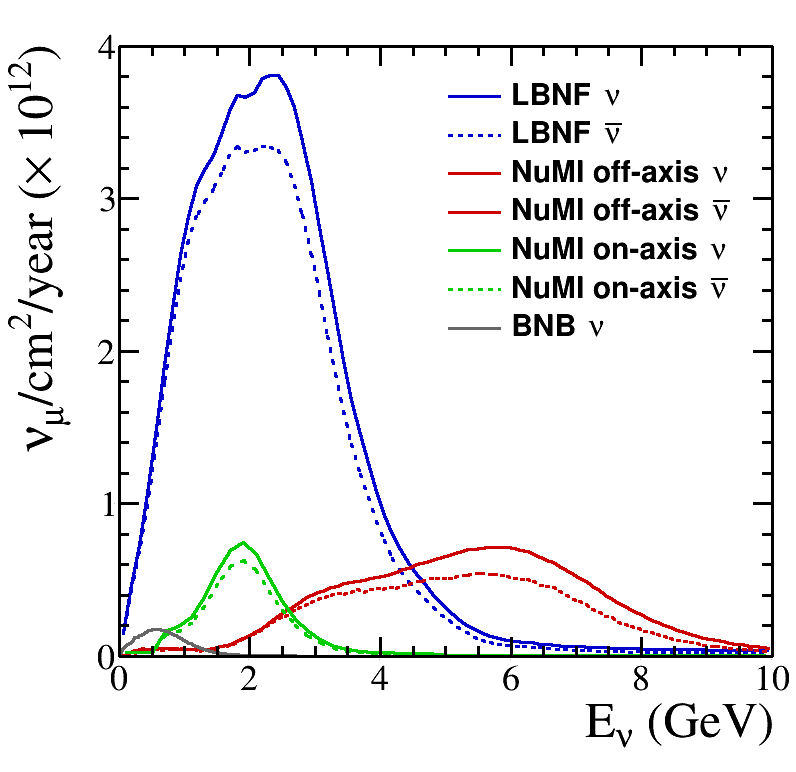
\includegraphics[width=0.5\textwidth]{plots/fnal_flux_comparison.png}}
  \subfloat[Rate\label{subfig:rate}]    {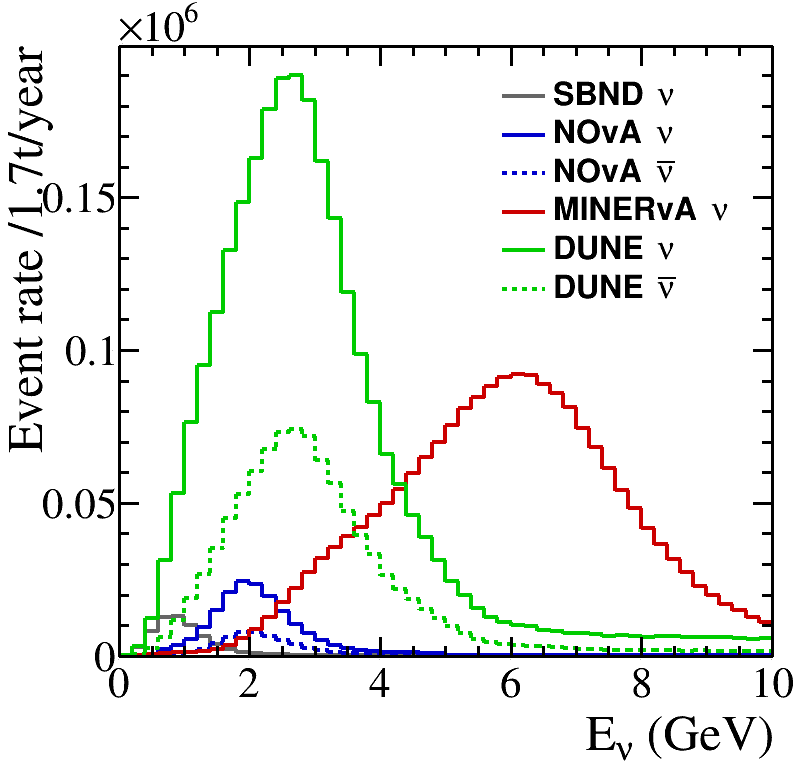
\includegraphics[width=0.5\textwidth]{plots/2x2_Enu_all.png}}
  \caption{Comparison of the absolutely normalized fluxes for different neutrino beamlines at Fermilab, and the expected yearly rates in a 1.7t LAr volume as a function of \enu, produced using GENIE v2.12.8 with the ValenciaQEBergerSehgalCOHRES configuration~\cite{genie}.}
  \label{fig:beam_options}
\end{figure}
In Figure~\ref{subfig:flux}, the currently available neutrino fluxes at various near detector halls in Fermilab are compared, on an absolutely normalized scale, to the LBNF three-horn optimized flux at the 574m near detector site~\addcite. The currently available neutrino fluxes considered are the on- and 14 mrad. off-axis medium-energy neutrinos from the main injector (NuMI) beam~\cite{numi}, which corresponds to the MINOS and NOvA near detector halls; and the booster neutrino beam (BNB) at the SBND hall~\addcite. The FY2017 delivered POT was used to produce a yearly flux and rate for the BNB and NuMI beams~\cite{fnal_beam_2017}. It is clear that the proposed LBNF flux is significantly more intense than the fluxes sampled at any existing experimental hall. However, due to the roughly linear relationship between neutrino energy and cross section, the measured rate from the on-axis NuMI beam in the MINOS-ND hall is approximately the same, and is therefore the most desirable currently functional experimental hall at Fermilab for a ProtoDUNE-ND test. The rate has been produced with the GENIE neutrino interaction Monte Carlo package~\cite{genie}, using v2.12.8 with the ValenciaQEBergerSehgalCOHRES configuration. Note that the rate is normalized to the active volume of the ArgonCube 2x2 Demonstrator module, showing that significant statistics will be accumulated in a matter of months of ProtoDUNE-ND operation.

\FloatBarrier
\subsection{MINOS near detector hall}
\label{sec:minos-hall}
\begin{itemize}
\item Size of the hall
\item Existing infrastructure required for the test
\item Need to consider whether we need to move anything (e.g. MINERvA) to make space
\item New infrastructure to be put in for the test --> Barry Norris/ Alan Bross. Probably need to discuss language with Steve Brice to make it forceful enough
\end{itemize}

\subsection{ArgonCube 2x2 demonstrator module}
\label{sec:2x2-design}
Callum/James

\subsection{3DST}
\label{sec:3dst-design}
Chang Kee?

\subsection{HPTPC}
\label{sec:hptpc-design}
Jen Raaf/Alan Bross?

